\documentclass[tikz,border=2pt]{standalone}
\usepackage{helvet}
\renewcommand{\familydefault}{\sfdefault}
\usetikzlibrary{arrows.meta,positioning,fit,calc,backgrounds}
\definecolor{ink}{HTML}{1F2933}
\definecolor{agent}{HTML}{E8F0FE}
\definecolor{agentb}{HTML}{3B6FD4}
\definecolor{graphc}{HTML}{FFF4DE}
\definecolor{graphb}{HTML}{C98A12}
\definecolor{alem}{HTML}{E6F6EC}
\definecolor{alemb}{HTML}{2E8B57}
\definecolor{art}{HTML}{F3E8FD}
\definecolor{artb}{HTML}{7B3FB5}
\definecolor{mute}{HTML}{6B7280}
\begin{document}
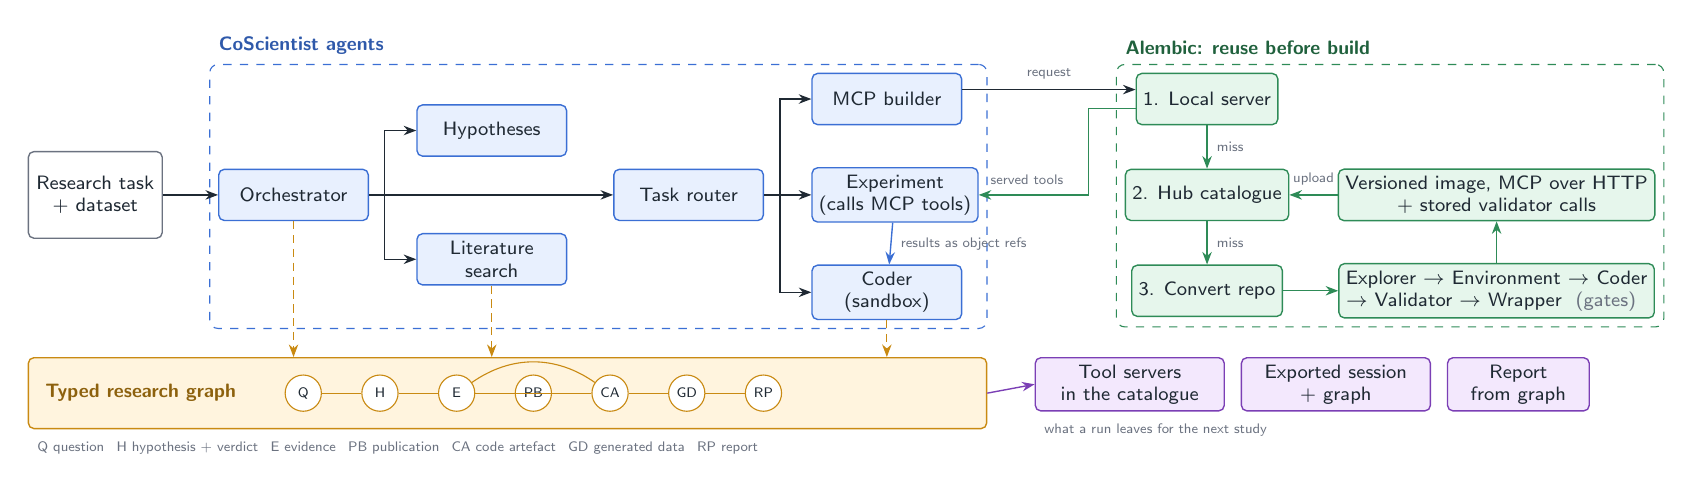
\begin{tikzpicture}[
  font=\scriptsize, text=ink, >={Stealth[length=1.6mm]},
  box/.style={draw=#1, line width=0.5pt, rounded corners=2pt, align=center, inner sep=2.5pt, minimum height=6.5mm},
  ag/.style={box=agentb, fill=agent, minimum width=19mm},
  al/.style={box=alemb, fill=alem, minimum width=17mm},
  ar/.style={box=artb, fill=art, minimum width=24mm},
  nd/.style={draw=graphb, fill=white, circle, inner sep=0.8pt, minimum size=4.6mm, font=\tiny},
  flow/.style={->, draw=ink, line width=0.5pt},
  wr/.style={->, draw=graphb, line width=0.4pt, densely dashed},
  lab/.style={font=\tiny, text=mute, align=center}
]
% ---- user
\node[box=mute, fill=white, minimum width=17mm, minimum height=11mm] (user) {Research task\\+ dataset};

% ---- agents
\node[ag, right=7mm of user] (orch) {Orchestrator};
\node[ag, above right=1.5mm and 6mm of orch] (hyp) {Hypotheses};
\node[ag, below right=1.5mm and 6mm of orch] (lit) {Literature\\search};
\node[ag, right=31mm of orch] (exec) {Task router};
\node[ag, above right=5.5mm and 6mm of exec] (mcpb) {MCP builder};
\node[ag, right=6mm of exec] (tool) {Experiment\\(calls MCP tools)};
\node[ag, below right=5.5mm and 6mm of exec] (coder) {Coder\\(sandbox)};

\draw[flow] (user) -- (orch);
\draw[flow] (orch.east) -- ++(2mm,0) |- (hyp.west);
\draw[flow] (orch.east) -- ++(2mm,0) |- (lit.west);
\draw[flow] (orch) -- (exec);
\draw[flow] (exec.east) -- ++(2mm,0) |- (mcpb.west);
\draw[flow] (exec) -- (tool);
\draw[flow] (exec.east) -- ++(2mm,0) |- (coder.west);
\draw[flow, draw=agentb] (tool) -- node[lab, right] {results as object refs} (coder);

% ---- research graph band
\path let \p1=(user.west), \p2=(coder.east) in
  node[box=graphb, fill=graphc, minimum height=9mm, anchor=north west, minimum width=\x2-\x1+3mm]
  (graph) at ($(user.south west)+(0,-15mm)$) {};
\node[anchor=west, font=\scriptsize\bfseries, text=graphb!70!black] at ($(graph.west)+(1mm,0)$) {Typed research graph};
\node[nd] (q)  at ($(graph.west)+(35mm,0)$) {Q};
\node[nd, right=5mm of q]  (h) {H};
\node[nd, right=5mm of h]  (e) {E};
\node[nd, right=5mm of e]  (p) {PB};
\node[nd, right=5mm of p]  (ca) {CA};
\node[nd, right=5mm of ca] (gd) {GD};
\node[nd, right=5mm of gd] (rp) {RP};
\foreach \a/\b in {q/h,h/e,e/p,e/ca,ca/gd,gd/rp} \draw[draw=graphb, line width=0.4pt] (\a) -- (\b);
\draw[draw=graphb, line width=0.4pt] (e) to[bend left=35] (ca);
\draw[wr] (orch.south) -- (orch.south |- graph.north);
\draw[wr] (lit.south) -- (lit.south |- graph.north);
\draw[wr] (coder.south) -- (coder.south |- graph.north);
\node[lab, anchor=north west] at ($(graph.south west)+(0,-0.3mm)$) {Q question \, H hypothesis + verdict \, E evidence \, PB publication \, CA code artefact \, GD generated data \, RP report};

% ---- alembic cascade
\node[al, right=22mm of mcpb]  (local) {1. Local server};
\node[al, below=5.5mm of local] (hub) {2. Hub catalogue};
\node[al, below=5.5mm of hub]  (build) {3. Convert repo};
\draw[flow, draw=alemb] (local) -- node[lab, right] {miss} (hub);
\draw[flow, draw=alemb] (hub) -- node[lab, right] {miss} (build);
\draw[flow] ($(mcpb.east)+(0,1.2mm)$) -- node[lab, above] {request} ($(local.west)+(0,1.2mm)$);
\draw[flow, draw=alemb] ($(local.west)+(0,-1.2mm)$) -- ++(-6mm,0) |- node[lab, pos=0.78, above] {served tools} (tool.east);
\node[al, right=7mm of build, minimum width=30mm, align=left] (stages)
  {Explorer $\to$ Environment $\to$ Coder\\$\to$ Validator $\to$ Wrapper \ \textcolor{mute}{(gates)}};
\draw[flow, draw=alemb] (build) -- (stages);
\node[al, minimum width=30mm] (img) at (stages |- hub) {Versioned image, MCP over HTTP\\+ stored validator calls};
\draw[flow, draw=alemb] (stages) -- (img);
\draw[flow, draw=alemb] (img) -- node[lab, above] {upload} (hub);
\begin{scope}[on background layer]
  \node[draw=alemb, dashed, rounded corners=3pt, inner sep=3pt, fit=(local)(hub)(build)(stages)(img),
        label={[font=\scriptsize\bfseries, text=alemb!70!black, anchor=south west]north west:Alembic: reuse before build}] (abox) {};
  \node[draw=agentb, dashed, rounded corners=3pt, inner sep=3pt, fit=(orch)(hyp)(lit)(exec)(tool)(coder)(mcpb),
        label={[font=\scriptsize\bfseries, text=agentb!80!black, anchor=south west]north west:CoScientist agents}] (cbox) {};
\end{scope}

% ---- artefacts
\node[ar, anchor=north west, minimum width=24mm] (a1) at ($(graph.north east)+(6mm,0)$) {Tool servers\\in the catalogue};
\node[ar, right=2mm of a1] (a2) {Exported session\\+ graph};
\node[ar, right=2mm of a2, minimum width=18mm] (a3) {Report\\from graph};
\node[lab, anchor=north west] at ($(a1.south west)+(0,-0.3mm)$) {what a run leaves for the next study};
\draw[flow, draw=artb] (graph.east) -- (a1.west);
\end{tikzpicture}
\end{document}
